% Partial sums S(x) = sum_{n <= x} chi_{-4}(n) Lambda(n)/n, at x = 10,20,...,80.
% Three-decimal values, rounded: -0.200, -0.209, -0.206, -0.219, -0.258, -0.252, -0.248, -0.304.
% Bars hang below zero. One unit of height is 0.10 in the sum.
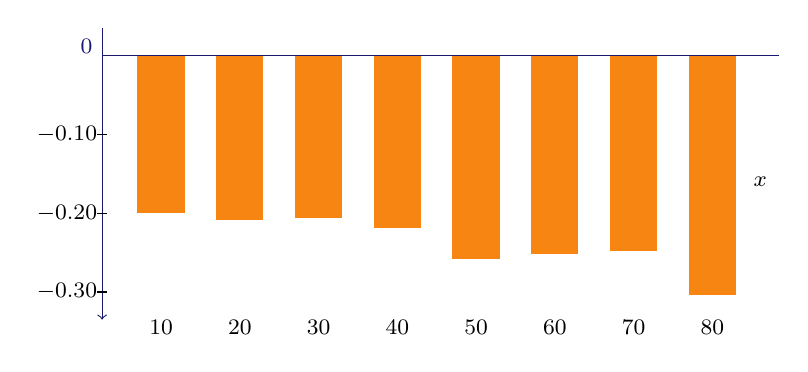
\begin{tikzpicture}[every node/.style={font=\footnotesize}]
  \draw[MidnightBlue] (0,0)--(8.6,0);
  \draw[->,MidnightBlue] (0,0.35)--(0,-3.35);
  \node[left,MidnightBlue] at (0,0.12) {$0$};
  \draw (-0.06,-1.0)--(0.06,-1.0) node[left] {$-0.10$};
  \draw (-0.06,-2.0)--(0.06,-2.0) node[left] {$-0.20$};
  \draw (-0.06,-3.0)--(0.06,-3.0) node[left] {$-0.30$};
  \fill[BurntOrange] (0.45,0) rectangle (1.05,-2.00);
  \fill[BurntOrange] (1.45,0) rectangle (2.05,-2.09);
  \fill[BurntOrange] (2.45,0) rectangle (3.05,-2.06);
  \fill[BurntOrange] (3.45,0) rectangle (4.05,-2.19);
  \fill[BurntOrange] (4.45,0) rectangle (5.05,-2.58);
  \fill[BurntOrange] (5.45,0) rectangle (6.05,-2.52);
  \fill[BurntOrange] (6.45,0) rectangle (7.05,-2.48);
  \fill[BurntOrange] (7.45,0) rectangle (8.05,-3.04);
  \node at (0.75,-3.45) {$10$};
  \node at (1.75,-3.45) {$20$};
  \node at (2.75,-3.45) {$30$};
  \node at (3.75,-3.45) {$40$};
  \node at (4.75,-3.45) {$50$};
  \node at (5.75,-3.45) {$60$};
  \node at (6.75,-3.45) {$70$};
  \node at (7.75,-3.45) {$80$};
  \node[right] at (8.15,-1.6) {$x$};
\end{tikzpicture}
